\documentclass[a4paper,11pt,english]{article}
\usepackage{.styles/basic}
\usepackage{.styles/envs}

%%%%%%% Title %%%%%%%%%%%%%%%%%%%%%%%%%%%
\title{\textbf{Algebraic Topology} - Exercise Sheet 1}
\author{Tor Gjone (2503108) \& Michele Lorenzi (3461634)}

%%%%%%% Definitions %%%%%%%%%%%%%%%%%%%%%

% Michele's stuff
% (I hope I don't break something...)
% (Most of the command are thought for livetexing but some became habits)
% ( :D don't worry. I'm a huge fan of shortcuts myself )

\makeatletter 
% \ni was used in the definitions of other commands. This is a solution
\newcommand{\@ni}{{n-1}}

\newcommand{\pin}{\pi_n(X,x_0)}
\newcommand{\pini}{\pi_\@ni(X,x_0)}
\newcommand{\pinr}{\pi_n(X,A,x_0)}
\newcommand{\pinir}{\pi_\@ni(X,A,x_0)}
\newcommand{\hn}{H_n(X;\Z)}
\newcommand{\hni}{H_\@ni(X;\Z)}
\newcommand{\hnr}{H_n(X,A;\Z)}
\newcommand{\hnir}{H_\@ni(X,A;\Z)}
\newcommand{\dn}{D^n}
\newcommand{\dni}{D^\@ni}
\newcommand{\sn}{S^n}
\newcommand{\sni}{S^{n-1}}
\newcommand{\sph}{(D^n,\de D^n)}
\newcommand{\sphi}{(D^\@ni,\de D^\@ni)}
\newcommand{\sm}{\smallsetminus}
\newcommand{\til}{\tilde}
\newcommand{\fa}{\;\;\forall}
\newcommand{\ul}[1]{\,\underline{#1}\,}
\newcommand{\ol}{\overline}
\newcommand{\nf}{\normalfont}
\newcommand{\xs}{{x_1,\dots,x_n}}
\newcommand{\xso}{{x_0,\dots,x_n}}
\newcommand{\nn}[2]{{{#1}_1,\dots,{#1}_{#2}}}
\newcommand{\nno}[2]{{{#1}_0,\dots,{#1}_{#2}}}
\newcommand{\nns}[3]{{{#1}_1\,{#2}\,\dots\,{#2}\,{#1}_{#3}}}
\newcommand{\nnso}[3]{{{#1}_0\,{#2}\,\dots\,{#2}\,{#1}_{#3}}}
\newcommand{\cb}[1]{\{#1\}}
\newcommand{\de}{\partial}
%\newcommand{\xto}[1]{\xrightarrow{#1}}
\newcommand{\hto}{\hookrightarrow}
\newcommand{\nii}{\@ni}
\newcommand{\cont}{\reflectbox{$\in$}}
\newcommand{\mi}{{m-1}}
\newcommand{\ki}{{k-1}}
\DeclareMathOperator{\colim}{colim}
\DeclareMathOperator{\tel}{tel}
\DeclareMathOperator{\proj}{proj}


% Tor's stuff
\newcommand{\oc}[1]{\overset{\circ}{#1}}
\newcommand{\into}{\hookrightarrow}
\newcommand{\nb}{\nabla}
\renewcommand{\hat}{\widehat}

\usepackage{scalerel,stackengine}
\stackMath
\renewcommand\widehat[1]{%
\savestack{\tmpbox}{\stretchto{%
  \scaleto{%
    \scalerel*[\widthof{\ensuremath{#1}}]{\kern.1pt\mathchar"0362\kern.1pt}%
    {\rule{0ex}{\textheight}}%WIDTH-LIMITED CIRCUMFLEX
  }{\textheight}% 
}{2.4ex}}%
\stackon[-6.9pt]{#1}{\tmpbox}%
}


\newcommand{\diagSquare}[8]{
\begin{tikzpicture}[node distance=2cm, auto]
\node (a)              { $ #5 $ };
\node (b) [right of=a] { $ #6 $ };
\node (c) [below of=a] { $ #7 $ };
\node (d) [right of=c] { $ #8 $ };
\draw[-to] (a) to node { $ #1 $ } (b);
\draw[-to] (a) to node { $ #2 $ } (c);
\draw[-to] (b) to node { $ #3 $ } (d);
\draw[-to] (c) to node { $ #4 $ } (d);
\end{tikzpicture}
}

\newcommand{\congto}{\xrightarrow{\cong}}
\newcommand{\incto}[1][]{ \xhookrightarrow{#1} }
\newcommand{\xto}[1]{\xrightarrow{#1}}

% Text key words
\newcommand{\tif}{\text{if }}
\newcommand{\tand}{\text{and }}
\newcommand{\tsince}{\text{since }}


% Projective spaces
\def\RP{\mathbb{RP}}
\def\CP{\mathbb{CP}}
\def\HP{\mathbb{HP}}

% Common Categories
\DeclareMathOperator{\Top}   {\bf Top}
\DeclareMathOperator{\Ab}    {\bf Ab}
\DeclareMathOperator{\Cat}   {\bf Cat}
\DeclareMathOperator{\CAT}   {\bf CAT}
\DeclareMathOperator{\Mod}   {\bf Mod}
\DeclareMathOperator{\Ring}  {\bf Ring}
\DeclareMathOperator{\Group} {\bf Group}
\DeclareMathOperator{\sSet}  {{\bf sSet}}

% Homological Algebra
\DeclareMathOperator{\Hom}   {Hom}
\DeclareMathOperator{\Tor}   {Tor}
\DeclareMathOperator{\Ext}   {Ext}

% Common Lie Groups 
\DeclareMathOperator{\GL}    {GL}
\DeclareMathOperator{\SU}    {SU}
\DeclareMathOperator{\U}     {U}
\DeclareMathOperator{\Sp}    {Sp}

% Maths Operators
\DeclareMathOperator{\pr}    {pr}
\DeclareMathOperator{\id}    {id}
\DeclareMathOperator{\Ker}   {Ker}
\DeclareMathOperator{\im}    {Im}

% Standard sets
\def \N {\mathbb{N}}
\def \Z {\mathbb{Z}}
\def \Q {\mathbb{Q}}
\def \R {\mathbb{R}}
\def \C {\mathbb{C}}
\def \H {\mathbb{H}}

\def \E {\mathbb{E}}
\def \Z {\mathbb{Z}}
\def \I {\mathbb{I}}
\def \J {\mathbb{J}}

% Vector calculus
\newcommand{\dif}[3][]{
	\ensuremath{\frac{d^{#1} {#2}}{d {#3}^{#1}}}}
\newcommand{\pdif}[3][]{
	\ensuremath{\frac{\partial^{#1} {#2}}{\partial {#3}^{#1}}}}

% Vectors and matrices
\newcommand{\mat}[1]{\begin{matrix} #1 \end{matrix}}
\newcommand{\pmat}[1]{\begin{pmatrix} #1 \end{pmatrix}}
\newcommand{\bmat}[1]{\begin{bmatrix} #1 \end{bmatrix}}

% Add space around the argument
\newcommand{\qq}[1]{\quad#1\quad}
\newcommand{\q}[1]{\:\:#1\:\:}

% Implications
\newcommand{\la} {\ensuremath{\Longleftarrow}}
\newcommand{\ra} {\ensuremath{\Longrightarrow}}
\newcommand{\lra}{\ensuremath{\Longleftrightarrow}}

\newcommand{\pwf}[1]{\begin{cases} #1 \end{cases}}

% Shorthand
\newcommand{\vphi}{\varphi}
\newcommand{\veps}{\varepsilon}

\newcommand{\<}[1]{\langle #1 \rangle}

% Notation
\newcommand{\wddef}[1]{\underline{#1}}
\newcommand{\pref}[1]{(\ref{#1})}

% Maths Operators
\theoremstyle{plain}
\theoremstyle{definition}
\newtheorem{thrm}{Theorem}[section]
\newtheorem{prop}[thrm]{Proposition}
\newtheorem{corol}[thrm]{Corollary}
\newtheorem{lemma}[thrm]{Lemma}

\newtheorem{defn}[thrm]{Definition}
\newtheorem{exmp}[thrm]{Example}
\newtheorem{clame}[thrm]{Clame}

\theoremstyle{remark}
% \newtheorem{remark}[thrm]{\normalfont\large\textit Remark}
\newtheorem{remark}[thrm]{Remark}
\newtheorem{note}[thrm]{Note}


\newSimpleHeaderEnvironment{exercise}{Exercise }

\newcommand{\pX}{\partial X}

\setlength{\parindent}{0cm}
\setlength{\parskip}{3pt}
%%%%%%%% Content %%%%%%%%%%%%%%%%%%%%%%%%
\begin{document}

\mmaketitle

\begin{exercise}[1]

\begin{comment}
    The argument I had in mind was induction on the number of cells of X, but not explicitly using a cofiber sequence. Suppose X is obtained from a subcomplex X' by attaching an n-cell. Given a map f : X ---> Y, induction implies that f is homotopic to a map whose restriction to X' is one of a finite number of possible maps g_1, … ,g_k : X' ---> Y. It suffices to show that for each g_i there are only finitely many possible extensions f : X ---> Y, up to homotopy. Fix one such extension f_0, and let f be any other extension. The compositions of f_0 and f with a characteristic map for the n-cell give maps D^n ---> Y that agree on S^{n-1}, so they give a "difference" map d(f,f_0) : S^n ---> Y. We will use the following elementary fact:

    Lemma: Suppose we are given two basepoint-preserving maps from S^n to a space Z that agree on a disk D^n containing the basepoint. Then if the two maps define the same element of pi_n(Z), they are homotopic by a homotopy that stays fixed on D^n.

    Thus if pi_n(Y) is finite, there are only finitely many choices for f, up to homotopy fixing X'.

    Allen Hatcher
\end{comment}

To prove that $[X,Y]$ is finite we will argue by induction on the total number of cells in $X$. For the initial step of the induction we consider $X$ to be a single $0$-cell. Then, fixing some arbitrary $y_0 \in Y$, we  have $[X,Y] \cong \pi_0(Y,y_0)$, which we 
assumed to be finite.

Now for the inductive step, we suppose that for the CW-complex $X'$ we have already proved that $[X',Y]$ is finite, and we want to show that if we get $X$ by attaching a singe $n$-cell $D$ to $X'$, then also $[X,Y]$ is finite.

Let $g : X' \to Y$, then we will denote by $(X,Y,g)$, the set of maps $f: X \to Y$ such that $f|_{X'} = g$. 
We will consider two maps in $(X,Y,g)$ to be homotopic if there exists a homotopy $H$ relative $X'$ between them, and call $[X,Y,g]$ be the set of homotopy classes in $(X,Y,g)$.

Let $g_1,\dots, g_k: X' \to Y$ represent the homotopy classes in $[X',Y]$ and let $f: X \to Y$. 
Since $f|_{X'}$ is a map from $X'$ to $Y$ we know that there must be a homotopy from $f|_{X'}$
to $g_i$, for some unique $i$. Clearly $(X,X')$ defines a relative CW-complex, so we may apply the 
homotopy extension property (HEP) to get a homotopy from $f$ to some map $f': X\to Y$, 
such that $f'|_{X'} = g_i$. So if we define the map
\[ \Psi : \bigsqcup_{j=0}^k [X,Y,g_j] \to [X,Y],\ [h] \to [h], \]
we have that $[f] \in \Psi([X,Y,g_i])$ (note that $\Phi$ is clearly well defined, since every homotopy relative $X'$ between two maps is in particular a homotopy between them). This means that the map $\Phi$ we defined is surjective (it is in fact a bijection, but we do not need this fact), so by showing that 
the left side is finite we may conclude that also the right side is finite, our goal.

Now to prove that $\bigsqcup_{i=0}^k [X,Y,g_i]$ is finite it suffices to show that each of the factors are finite. Fix a point $x_0 \in X'$, on the boundary of the $n$-cell $D$ that we need to attach to get $X$. We suppose without loss of generality that $[X,Y,g_i]$ is non-empty and we fix an element $f_0 \in (X,Y,g_i)$.

To show that $[X,Y,g_i]$ is finite we will define a map $d: [X,Y,g_i] \to \pi_n(Y,y_0)$, where $y_0 = g_i(x_0)$, that 
can be thought of as the "difference" between $f$ and $f_0$, for some $f\in(X,Y,g_i)$.

We consider $S^n$ to be the union of two copies of the $n$-disk $D^n$, glued together on the boundaries, i.e. 
$S^n = D^n \sqcup_\partial D^n$. For $f \in (X,Y,g_i)$ we define d([f]) := [d(f)] (by slight abuse of notation),
where $d(f): S^n = D^n \sqcup_\partial D^n \to Y$ is defined by
\[ d(f)|_{\text{first factor}} = f_0|_{D^n} \q{\text{and}} d(f)|_{\text{second factor}} = f|_{D^n}, \]
where the $D^n$ on the right side of the equations refers to the $n$-cell (i.e. $\cong D^n$) that was attached to $X'$ to get $X$.

We need to check that this is well-defined. Suppose $f$ and $g$ are homotopic, by $H$ say, in $(X,Y,g_i)$, then $H|_{D^n}$ defines a homotopy from $f|_{D^n}$ to $g|_{D^n}$
that is fixed on the boundary. We define $H': S^n\times I \to Y$, by $H'|_{\text{first factor}} = H|_{D^n}$ and constant on the second 
factor. Then $H'$ defines a homotopy from $d(f)$ to $d(g)$, and thus $d$ is well-defined.

Finally we will show that $d$ is injective, which finishes the proof, since $\pi_n(Y,y_0)$ is finite. Suppose $d(f)$ and $d(g)$ are homotopic as based maps from $S^n$ to $Y$, by a homotopy $H$ say. 
Since they agree on a disk containing the basepoint, we can define a homotopy $H'$ relative a hemi-sphere $D^n$ between them: this can be done by concatenating three homotopies, first a expansion of the base point to a hemi-sphere (a contraction in reverse), then a homotopy which is $H$ on the other hemi-sphere and constant on the "expanded" hemi-sphere, then a contraction of the hemisphere to the basepoint.

\textbf{Warning!}
The argument for injectivity of $d$ is clearly faulty as it stands and we do not have time left to find an alternative, but since we think it could be salvaged and made into an actual proof we are leaving it as it is.

Again we consider $S^n$ to be the union on two disks. Then $H'$ restricted to the second defines a homotopy between $f|_{D^n}$ and $g|_{D^n}$. By extending this homotopy to $X$ we get a homotopy from $f$ to $g$ in $(X,Y,g_i)$.

%Now, suppose we are given two basepoint-preserving maps from $S^n$ to a space $Z$ that agree on a disk $D^n$ containing the basepoint. Then if the two maps define the same element of $\pi_n(Z)$, they are homotopic by a homotopy that stays fixed on $D^n$.

\end{exercise} 



\begin{comment}
We will be doing the proof in a number of steps.
\begin{itemize}
\item Suppose for now that we have already proved the statement for $Y$
path-connected. Let $X^i \subset X$,  denote the path-connected components of $X$ and
similarly $Y^j \subset Y$ the path-connected components of $Y$. Then, by
assumption, $[X^i,Y^j]$, the set of homotopy classes of maps from $X^i$ to
$Y^j$, is finite.
Consider a map $f: X \to Y$, then for each $X^i\subset X$, $f|_{X^i}$ most be
contained in one of the path-connected components of $Y$, say $Y^j$. So
$f|_{X^i}$ defines an element in $[f|_{X^i}^{Y^j}] \in [X^i, Y^j]$.
Define the following map
\[ \Phi : [X, Y] \to \prod_{i, j} \left( [X^i, Y^j] \sqcup \{ \omega \} \right);
\quad 
f \mapsto \prod{i,j} [f|_{X^i}^{Y^j}], \]
where $[f|_{X^i}^{Y^j}] = \omega$, whenever $f(X^i) \cap Y^j = \emptyset$. We
want to show that this map is well-defined and injective, because if it is $[X,
Y]$ most be fine, since the co-domain is a finite product of finite elements and
thus finite.
\item Suppose $f, g: X \to Y$ are homotopy equivalent by some homotopy $H$, then
$H|_{X^i}$ defines a homotopy from $f|_{X^i}$ to $g|_{X^i}$. So $\Phi$ is
well-defined. 
\item Now suppose $f,g: X \to Y$ such that $\Phi([f]) = \Phi([g])$. Then $f|_X^i$ is
homotopy equivalent to $g|_{X^i}$ by some homotopy $H_i$ for all of the
path-connected components of $X$. Clearly we may defined $H: I\times X \to Y$
by $H|_{X_i} = H_i$, which defines a homotopy between $f$ and $g$.
\item So we may now, in the more interesting part of the proof, suppose wlog. that
$Y$ is path-connected. The idea of the proof is to consider another set of
homotopy classes, that projects surjective onto $[X,Y]$, and show that this set
is finite, which would imply that $[X,Y]$ is also finite.
\item Fix an element $y_0 \in Y$ and let $\pX \subset X$ denote the set of boundaries
in $X$, ie. $x \in \pX$ if and only if $x \in \partial D^i$ for some $i$-cell in
$X$.
Let $(X,Y,y_0)$ denote the set of of maps $f: X \to Y$, such that $f(\pX) = \{
y_0\}$ (or alternatively, such that for any $i$-cell $D^i$ in $X$, $f(\partial
D^i) = \{ y_0 \}$. ) 
Let $f, g \in (X,Y,y_0)$, then a homotopy between $f$ and $g$ is a homotopy $H:
I \times X \to Y$ (ie. $H(0,-) = f$ and $H(1,-) = g$) such that $H(I, \pX) = \{
y_0 \}$. Then we will let $[X,Y,y_0]$ be the set of homotopy classes in 
$(X,Y,y_0)$.
\item We will now prove that $[X,Y,y_0]$ is finite. 
Like above the strategy will be to construct a map from $[X,Y,y_0]$ into something 
finite and show that the map is injective. Let $f \in (X,Y,y_0)$ and $D_i \subset X$
be an $i$-cell. Then, since $f(\partial D^i) = \{ y_0 \}$, there is a unique based 
map $\tilde{f}_{D^i} : (S^1, x_0) \to (Y, y_0)$, such that $f|_{D^i}$ factors though
$\tilde{f}_{D^i}$. (ie. $f|_{D^i} = \tilde{f}_{D^i} \circ q$, where $q : D^i \to S^i$
is the quotation map, that send the boundary $\partial D^i$ to $x_0$). We define
\[ \Psi : [X,Y,y_0] \to \prod_{D^i \:i\text{-cell in } X} \pi_i(Y, y_0); \quad
[f] \mapsto [\tilde{f}_{D^i}]. \]
\item Firstly we will need to show that this is well-defined. Suppose $H$ defines an 
homotopy between $f$ and $g$ in $(X,Y,y_0)$. Then for each $D^i$, $H|_{D^i}$ defines 
a homotopy between $f|_{D^i}$ and $g|_{D^i}$, such that $H(I,\partial D^i) = {y_0}$. 
Clearly this homotopy descends to the quotient $D^i / \partial D^i$ and thus defines
a homotopy between $\tilde{f}_{D_i}$ and $\tilde{g}_{D^i}$. 
\item To show that $\Psi$ is injective, suppose $f,g \in (X,Y,y_0)$ such that 
$[\tilde{f}_{D^i}] = [\tilde{g}_{D^i}]$ for all $D^i$ $i$-cells in $X$. That is for 
all $D^i$, there exists a based homotopy $\tilde{H}_{D^i}: I \times S^i \to Y$ between
$\tilde{f}_{D^i}$ and $\tilde{g}_{D^i}$. By associating $S^i$ with $D^i/\partial D^i$, 
we may define $H_{D^i}: I \times D^i \to Y$ by 
$H_{D^i}|_{\mathring{D^i}} = \tilde{H}_{D^i}|_{\mathring{D^i}}$  and 
$H_{D^i}|_{\partial D^i} = \tilde{H}_{D^i}|_{\partial D^i}$. 
Finally define $H: I\times X \to Y$ by $H|_{D^i} = H_{D^i}$, which is well-defined 
since the cells only intersect on the boundaries which are all sent to the same point.
So $f$ and $g$ are homotopic by $H$, in $(X,Y,y_0)$ and thus $[f] = [g]$.
\item Now that we have shown that $[X,Y,y_0]$ is finite, we need to show that this implies 
$[X,Y]$ is finite. We will do this by induction on the cells of $X$.
We will start the induction with the sub CW-complex $X_1$, given by the $1$-skeletal, 
of $X$.
In this case we can for any $f: X_1 \to Y$ find a homotopy from $f$ to a
map $\tilde{f} \in (X,Y,y_0)$
Suppose $X$ is obtained from a sub complex $X'$
\item We now claim that for any map $f: X \to Y$ there exists a map $\tilde{f} \in
[f]$ such that $\tilde{f} \in (X, Y, y_0)$. We will come back to the proof of
the claim further down, but for now will take it to be true. Clearly every map
in $(X,Y,y_0)$ is in particular a map from $X \to Y$, so we may define a map $p
: (X,Y,y_0) \to [X,Y]$. Also every homotopy that fixes $\pX$ is in particular a
homotopy, so $p$ descends to define a map $p_* : [X,Y,y_0] \to [X,Y]$. Finally
the claim implies that this map $p_*$ is in fact surjective.
\item It still remains to prove the claim above that any map $f : X \to Y$ is homotopic
to a map $\tilde{f} \in (X,Y,y_0)$. To construct $\tilde{f}$, we will construct a 
homotopy from $f$ by applying the homotopy extensions properly (HEP) over and over 
starting by sending the pints in $X_0$ to $y_0$. 
Since $Y$ is path-connected there exists for every point $x_i \in X_0$ a path 
$\phi_i$ from $f(x_i)$ to $y_0$ in $Y$. We define $H_0 : I \times X_0 \to Y$
by $H_0(t,x_i) = \phi_i(x_i)$. Then $H_0$ defines a homotopy between 
$f|_{X_0}$ and the constant map from $X_0$ to $y_0$. Since $X_0$ is a sub
CW-complex of $X$, the pair $(X, X_0)$ clearly defines a relative CW-complex,
so it has the HEP. Define $H_1 : I\times X\to Y$, by the HEP, such that 
$H_1|_{X_0} = H_0$ and $H_1(0, -) = f$.
Let $f_1 = H_1(1, -)$. We observe that, since $f_1(X_0) = H_1(1,X_0) = \{ y_0 \}$, 
we have that for any $D^1$ $1$-cell in $X$, $f_1(\partial D^1) \subset 
f_1(X_0) = \{ y_0 \}$.
To construct the final $H$, we will inductively define $H_n$ (and $f_n = H(1,-)$,) such that 
$H_n(1, \partial D^i) = \{ y_0 \}$ for all $D^i$ $i$-cells, for all $i \le n$. 
The case $n=1$ we have already done, so we suppose that we have already constructed 
$H_{n-1}$, with the desired property.
For the inductive step we will construct $H_n$ by induction on the $n$-cells.
Let $(D_j)_{j=1}^k$ denote the collection of $n$-cells in $X$. Then we will define 
homotopies $H_n^{j}$, such that $H_n^j(1, -)$ maps all $i$-cells, for $i<n$, and all 
$n$ cells $D_i$, for $i \le j$, to $y_0$, and $H_n^j(0,-) = H_n^{j-1}(1,-)$. 
We define $H_n^0 = H_{n-1}$. So assuming we have done the induction already, we
may defining $H_n$ to be the concatenation of all the $H_n^j$'s we get the desired 
homotopy.
Since we have defined $H_n^0$ to be $H_{n-1}$, the initial case of the 
induction is trivial. For the inductive strep we suppose we have already defined
$H_n^{j-1}$. If the boundary of $D_j$ is already mapped to $y_0$, we may simply define 
$H_n^j$ to be the homotopy, defined by $H_n^j(t, -) = f_n^{j-1} := H_n^{j-1}(1, -)$,
for all $t \in I$. 
Suppose $D_j$ is not mapped to $y_0$. Then 
This does not work!!!
\end{itemize}
\end{comment}



\begin{exercise}[2]

$(a)$ Consider $S^n$ with the CW-structure given by attaching two $n$-cells to $S^\nii$. Let $p$ be the quotient map $S^n\to S^n/S^\nii$. The quotient $S^n/S^\nii$ inherits a CW-structure consisting of one $0$-cell and two $n$-cells attached to it, i.e. it is the wedge of two $n$-spheres $S^n\vee S^n$. Clearly $p$ is continuous and the composition $q_1\circ p$ is the quotient map $S^n\to S^n$ sending an hemi-sphere of $S^n$ (i.e. $S^\nii$ and one of the two $n$-cells attached to it) to the $0$-cell of $S^n$ (with the CW-structure consisting of two cells, one $0$-cell and one $n$-cell). Now, since hemi-spheres are contractible, we can construct an homotopy between such a map and the identity. \bigskip

$(b)$ Consider the diagram:
\begin{center}
    \begin{tikzcd}
    H_n(S^n;A) \arrow[r, "p_*"] & H_n(S^n\vee S^n;A)\cong H_n(S^n;A)\oplus H_n(S^n;A) \arrow[r, "(i_1\vee i_2)_*"] & H_n(S^n\vee S^n;A) 
    \end{tikzcd}
\end{center}
where the isomorphism $H_n(S^n\vee S^n;A)\to H_n(S^n;A)\oplus H_n(S^n;A)$ is given by $q_{1*}\oplus q_{2*}$ (the inverse of ($i_{1*}+i_{2*}$), and this holds for all coefficient groups $A$). In particular we have:
\begin{align*}
    ((i_1\vee i_2)\circ p)_* &= (i_1\vee i_2)_*\circ (i_{1*}+i_{2*}) \circ (q_{1*}\oplus q_{2*}) \circ p_* \\
    &= ((i_1\vee i_2)_*\circ i_{1*} \circ q_{1*} \circ p_*) + ((i_1\vee i_2)_*\circ i_{2*} \circ q_{2*} \circ p_*) \\
    &= ((i_1\vee i_2)_*\circ i_{1*}) + ((i_1\vee i_2)_*\circ i_{2*}) = i_{1*} + i_{2*}
\end{align*}
where we used that $i_1\circ q_2$ and $i_2\circ q_1$ are constant maps (hence they induce the zero map on homology), that $q_1\circ p$ and $q_2\circ p$ are homotopic to the identity (hence they induce the identity on homology), and that $(i_1\vee i_2)\circ i_1=i_1$ and $(i_1\vee i_2)\circ i_2=i_2$. \bigskip

$(c)$ The Hurewicz theorem tells us that the Hurewicz map $h:\pi_n(S^n\vee S^n,x_0)\to H_n(S^n\vee S^n;\Z)$ is an isomorphism (note that $H_k(S^n\vee S^n;\Z)=H_k(S_n;\Z)\oplus H_k(S_n;\Z)=0$ for $k<n$). Now, given any two pinch maps $p$ and $\til{p}$, point $(b)$ tells us that \[h([p])=p_*(c)=(i_1)_*(c)+(i_2)_*(c)=\til{p}_*(c)=h([\til{p}])\]
i.e. their homotopy classes have the same image under the Hurewicz map. Since the Hurewicz map is an isomorphism, this means that $[p]$ and $[\til{p}]$ are the same element in $\pi_n(S^n\vee S^n,x_0)$, therefore $p$ and $\til{p}$ are homotopic as based maps.

\end{exercise}


\newpage
\begin{exercise}[3]

Note that in the second lecture we proved that if $(X,A)$ is a pair of path-connected spaces and $n\geq2$, then the "forgetful" homomorphism $\pinr^\dagger\to\pi_n(X,A)^\#$ is an isomorphism. This clearly implies that $\pi_2(X,A,x_0)^\dagger$ is an abelian group (since $\pi_n(X,A)^\#$ is just a quotient of a free abelian group).

To show that $\pi_2(X,A,x_0)^\dagger$ is abelian it is also possible to take a different route: there is a homotopy between $gfg^{-1}$ and $(\de g)*f$ (Where $\de g$ is a loop in $A$), which can be constructed as indicated by the following picture:\vspace{-0.3cm}
\begin{center}
    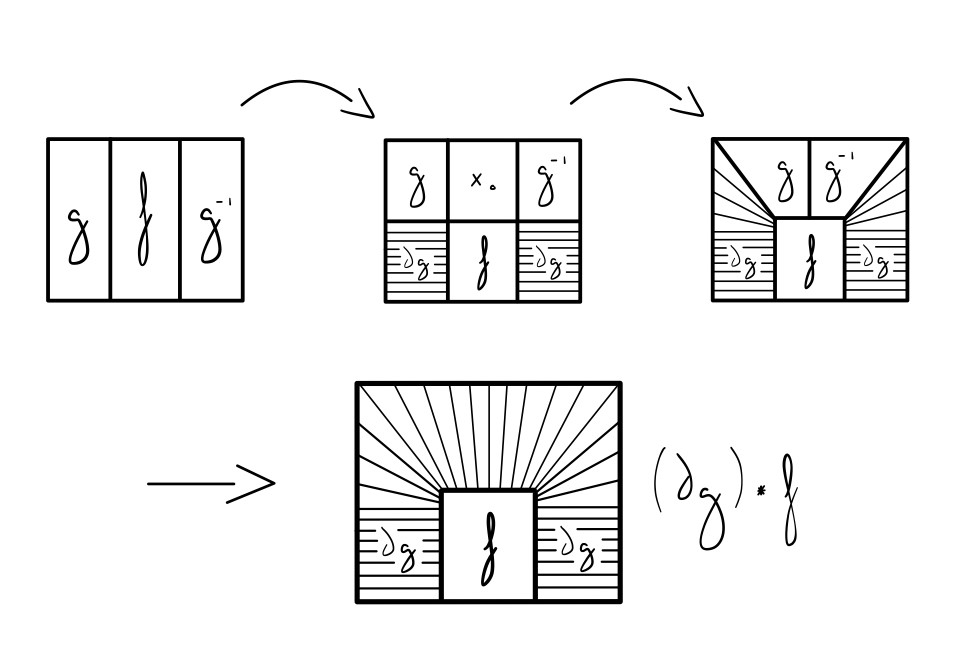
\includegraphics[scale=0.38]{Some_homotopy.jpg}
\end{center}
this means that $gfg^{-1}f^{-1}=((\de g)*f)f^{-1}$ in $\pi_2(X,A,x_0)$, that is $fg=gf$ in $\pi_2(X,A,x_0)^\dagger$.

\end{exercise}

\end{document}
